\documentclass[12pt, fullpage,letterpaper]{article}

% I copied older latex files that include packages we may need but idk,
% I'm not too knowledgeable about all things Latex
\usepackage[margin=1in]{geometry}
\usepackage{url}
\usepackage{amsmath}
\usepackage{amssymb}
\usepackage{xspace}
\usepackage{graphicx}
\usepackage{hyperref}
\usepackage{listings}
\usepackage{bm}
\usepackage{cite}
\usepackage{subfigure}

\graphicspath{{./}}
\title{Final Report}
\author{Tyler Adams: u0761872 \\Corbin Baldwin: u0292800}

\begin{document}
	\maketitle 
	\hrule 
	\vskip 0.5cm
	\section{Grading Rubric}
	\begin{enumerate}
		\item Team Members:  the names and UID of your team members.
		\item Introduction:  Motivation  and  a  brief  project  description.   What  is  the  main  objective  of  your project?  What is an overview of your strategy to achieve your objective?
		\item Technical Contributions:  What are the technical contributions of your proposed work?
		\item Data:  What are the type(s) of data your project will be dealing with?  How do you plan to gethold of such data sets?  What kind of insights are you planning to obtain from your data?
		\item Background and Related Work:  technical background, together with related work.  What are thestate-of-the-art techniques in dealing with the data of your interest?  What are the differences andsimilarities between your work and the state-of-the-art?
		\item Methods:   What  methods  have  you  used/developed?   What  are  your  strategies  in  tackling  the proposed problem?
		\item Results and Insights:  What are the results of your proposed project?  What are the key insights?
		\item Evaluation:  What metrics do you use to evaluate how successful your project is?  What are thetake home messages based on your evaluation?
		\item Deliverables:  What are your deliverables?  (e.g.  source code,  video demo,  etc.)  What software(and possibly hardware) do you use?  Or in the case you are working on software extensions, whatis the baseline software you work with?
		\item Conclusions and Dicussions:  answer specific questions below using 1-2 sentences:
		\begin{itemize}
			\item What is an overview of your project?
			\item What are your project objectives?
			\item What questions does your project address?
			\item What are the key insights based on your results?
			\item What are future directions?
		\end{itemize}
	\end{enumerate}	
	
	\section*{\normalfont Introduction}
	% Motivation and a brief project description.
	Rayleigh-Taylor instability (RTI) forms at the surface of contact between two fluids, one of which is denser and accelerates toward the other. Formations in RTI are not symmetric between the denser and lighter fluids, and the features of both sides serve to characterize the RTI. However, these features quickly rise in complexity, and it is unrealistic to simulate them beyond a given time threshold. In our project we hope to provide insights regarding structure that apply to RTI generally, including in the later stages of RTI development, using TDA methods.
	
	\section*{\normalfont Completed Milestones} We have successfully been able to install and run software that simulates RTI and saves the time-steps in 2D images which we can use further down the pipeline. Additionally, we have written software that extracts the isosurfaces of the images with which we can track bubble evolution and we have written software that smooths out noise using a regularized least squares method. Lastly we have also installed recommended software and were able to get the examples running on Morse-Smale complex computations. For more information on these divergent paths, see the Modifications section. An example time evolution is shown below.
%		\begin{figure*}[ht!]
%		\centering
%		\begin{subfigure}
%			\centering
%			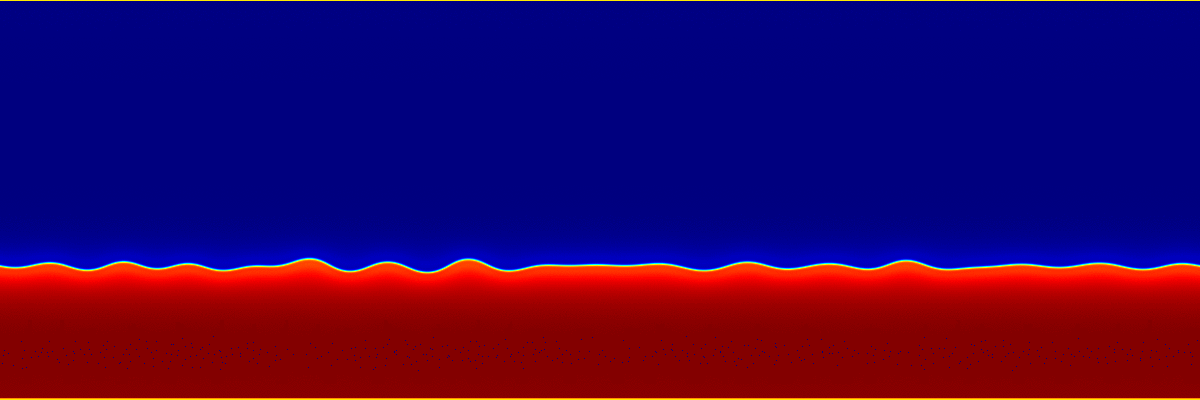
\includegraphics[scale = .25]{fig1.png}
%			\caption{$t = 2100$}
%		\end{subfigure}
%		\begin{subfigure}
%			\centering
%			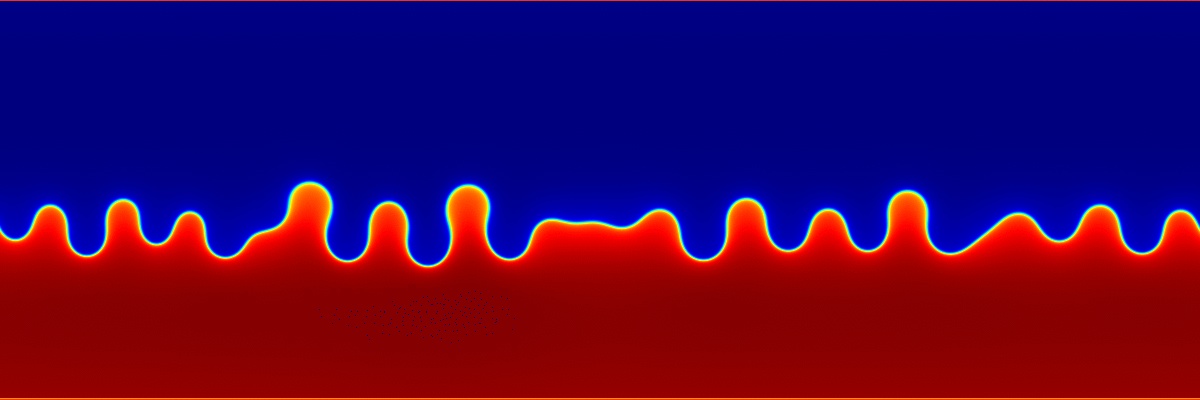
\includegraphics[scale = .25]{fig2.png}
%			\caption{$t = 2600$}
%		\end{subfigure}
%		\begin{subfigure}
%			\centering
%			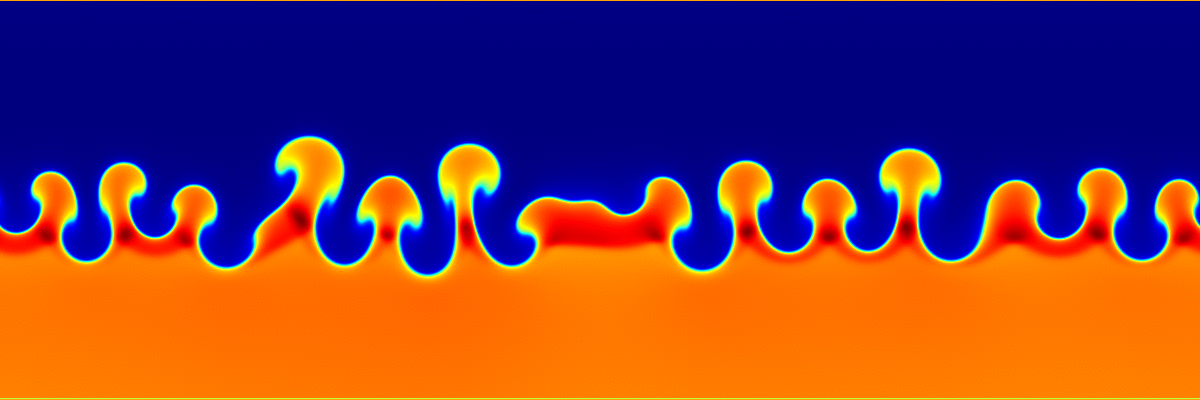
\includegraphics[scale = .25]{fig3.png}
%			\caption{$t = 2900$}
%		\end{subfigure}
%		\begin{subfigure}
%			\centering
%			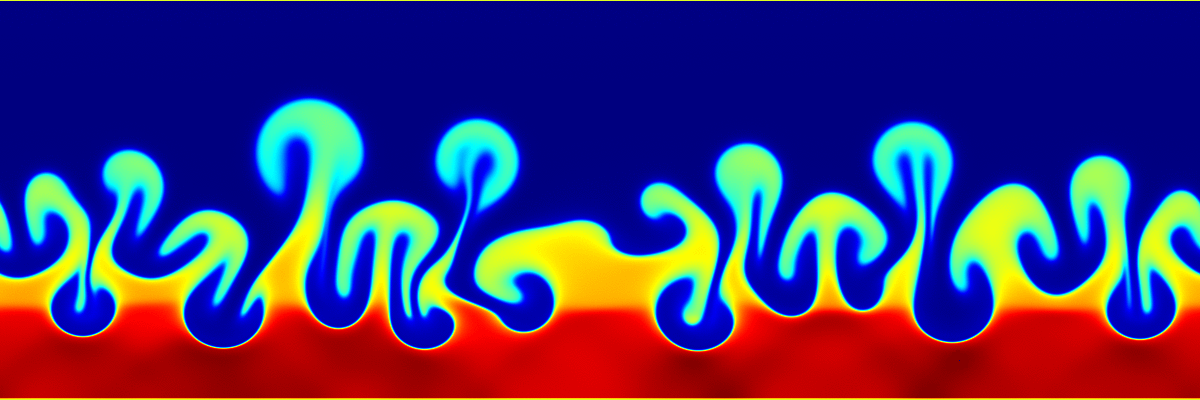
\includegraphics[scale = .25]{fig4.png}
%			\caption{$t = 3300$}
%		\end{subfigure}
%	\end{figure*}
%	
	
	\section*{\normalfont Upcoming Milestones} The next milestones are:
	\begin{enumerate}
%		\item Smooth out the isosurfaces so that we can better track bubble evolution.
		\item Implement a height function to track critical points and the evolution of bubbles.
		\item Construct a persistence diagram describing the birth and death of bubbles.
		\item Possibly classify simulations by density or other parameters by their persistence diagrams. I.e., is this bubble evolution symptomatic of the mixing of air and water?
	\end{enumerate} 

	\section*{\normalfont Preliminary Results}
	While we have not applied a proper topological filtration, we have extracted some data that will be necessary in the final stages. The most challenging aspect so far has been finding a valid, practical algorithm for running the simulation of an RTI. As shown above, we have managed to get one working that provides a solution to the problem in the two dimensional case. With the images that are output, we can approximate the isosurface using edge-detecting algorithms, which we have also done.
	
	\section*{\normalfont Modifications} RTI is a difficult to simulate on a large scale as it involves numerically solving the system of PDE's
	
	\begin{gather*}
		\frac{\partial \rho Y_i}{\partial t} + \nabla \cdot (\rho Y_i \vec{u} + \vec{J}_i) = 0; i = 1, 2 \\
		\frac{\partial \rho \vec{u}}{\partial t} + \nabla \cdot (\rho \vec{u} \cdot \vec{u} + p \vec{\vec{\delta}} - \vec{\vec{\tau}}) = \rho \vec{g} \\
		\frac{\partial E}{\partial t} + \nabla \cdot ((E + p)\vec{u} -\vec{\vec{\tau}}\cdot \vec{u} + \vec{q_c} + \vec{q_d} ) = \rho \vec{g} \cdot \vec{u} \\
	\end{gather*} 
	at each time step. While we have some background in PDE's, we do not feel our background is sufficient to construct a solver from scratch quickly. After researching a few algorithms and trying to implement broken software, we found the Palabos library, located at \url{http://www.palabos.org/}, which contains the software used to generate the images above. Due to the computation intensive process of generating a 3D dataset on which to use Morse-Smale complexes, we may choose to use the 2-dimensional version. If we use 2D, we will use a height function to compute and store relevant critical point information. Additionally, since we are in essence extracting a boundary from the 2D sample image, we can use methods learned in this class to attempt to classify different mixing species using TDA and machine-learning. Alternatively, if we can generate sufficient 3D data, we can use the recommended software to continue with the project as originally planned.
	
	 	\section*{\normalfont Summary}
	We have arranged a process to acquire the data necessary for our research over two dimensional RTIs, including the simulation and the extraction of isosurfaces from said simulation. We hope to acquire three dimensional RTI data as well. Regarding the data, we still have not utilized topological data analysis to perform the essence of our research. This should include several topological filtrations.
	
	With the filtrations we plan to classify simulations by the structure of their RTIs. Factors that will be considered include the birth and death times of bubbles, as well as their size.


\end{document}
